\documentclass[]{article}

\usepackage[spanish]{babel}
\usepackage{graphicx}
\usepackage{amsmath,bm,amssymb,amsfonts}
\usepackage{algorithmic}

%opening
\title{}
\author{}

\begin{document}

\maketitle

\begin{abstract}

\end{abstract}

\section{Fundamentos Teóricos del Material}
	\subsection{Regresión Lineal por Mínimos Cuadrados}
	La Regresión Lineal por Mínimos Cuadrados (RLMC) es una técnica estadística y un algoritmo de aprendizaje automático supervisado, ampliamente utilizado para modelar la relación lineal entre una variable dependiente (salida, Y) y una o más variables independientes (entrada, X). Su objetivo primordial es encontrar la "línea de mejor ajuste" que represente esta relación, minimizando la suma de los cuadrados de las diferencias entre los valores observados y los valores predichos por el modelo. Estas diferencias son conocidas como residuos o errores.\\
	Como algoritmo predictivo, la RLMC establece una relación lineal entre la predicción (Y) y los datos (X), lo que se traduce en una línea recta si se representa gráficamente (Kaware S., 2021).

	\begin{figure}[h]
		\centering
		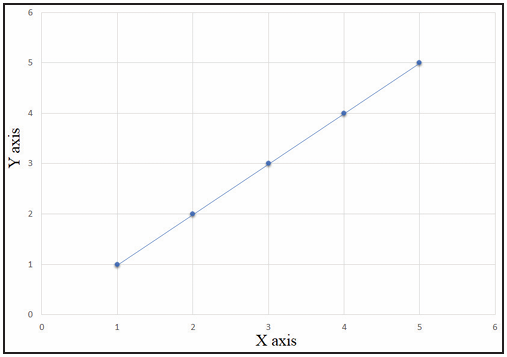
\includegraphics[width=0.7\linewidth]{imagenes/Imagen1}
		\caption{Representación de una ecuación lineal.}
		\label{fig:Imagen1}
	\end{figure}
	
		\subsubsection{Principios Fundamentales del Álgebra Lineal en RLMC}
		El álgebra lineal constituye la base matemática esencial para la Regresión Lineal por Mínimos Cuadrados y, de hecho, para gran parte del aprendizaje automático. Permite representar y manipular eficientemente grandes conjuntos de datos y las relaciones lineales entre variables (Watson, 1967).\\
		El álgebra lineal es reiteradamente identificada como la ``base'' y el ``núcleo'' para el aprendizaje automático, facilitando la implementación y siendo crucial para los ingenieros experimentados. La profunda integración del álgebra lineal no es meramente una conveniencia, sino una necesidad fundamental para el campo. Los algoritmos de aprendizaje automático, incluyendo la RLMC, operan intrínsecamente sobre datos que son, por naturaleza, multidimensionales, compuestos por características y observaciones. El álgebra lineal proporciona las herramientas esenciales, como vectores y matrices, para representar estos datos de manera estructurada y compacta. Las operaciones fundamentales en el aprendizaje automático, tales como la transformación de datos, el cálculo de distancias y la optimización de funciones de costo, se traducen directamente en operaciones de álgebra lineal, incluyendo la multiplicación de matrices, la inversión de matrices y el cálculo de gradientes (Andrade-Garda \& Carlosena-Zubieta, 2013).\\
		\\
		La formulación matricial de la RLMC, expresada por la ecuación:\\
		\[
		\hat{\bm{\beta}} = (X'X)^{-1} X'Y
		\]
		Es un ejemplo elocuente de cómo el álgebra lineal ofrece una solución analítica elegante y eficiente para la estimación de los parámetros del modelo. Esta capacidad para formular problemas complejos en términos de álgebra lineal permite la escalabilidad de los algoritmos a grandes conjuntos de datos, la derivación de soluciones analíticas para problemas de optimización y la conceptualización de modelos complejos de manera abstracta pero rigurosa. Para un profesional del aprendizaje automático, un dominio sólido del álgebra lineal no es un conocimiento adicional, sino una capacidad crítica para comprender, implementar y desarrollar nuevos modelos de manera efectiva (Andrade-Garda \& Carlosena-Zubieta, 2013).
		\\
		
\section{Aplicación del Material}
	\subsection{Proceso de Estimación de la Regresión por Mínimos Cuadrados}
	El método de mínimos cuadrados es una técnica estadística que minimiza el error, asegurando que la suma de todos los errores al cuadrado sea la mínima posible. La estimación de los coeficientes de la línea de regresión (pendiente y el intercepto) se puede realizar de forma analítica (Watson, 1967).\\
	En el contexto del artículo ``A Model Based Linear Algebraic Approach for Machine Learning'', el método de mínimos cuadrados implica ajustar un modelo a un conjunto de datos médicos relacionados con la pandemia del COVID-19, minimizando la suma de las diferencias al cuadrado entre los valores observados y los valores predichos. La línea o curva que minimiza esta suma se considera la línea o curva de mejor ajuste. El objetivo principal de este método es minimizar la suma de los residuos al cuadrado (Kaware S., 2021).\\
	\\
	Fórmula general de regresión lineal simple:
	\[
	 Y' = mx + b 
	\]
	\\
	Dónde:
	\[
	m = \frac{n \sum xy - \sum x \sum y}{n \sum x^{2} - (\sum x)^2}
	\]
	\\
	Y:
	\[
	b = \frac{\sum y}{n} - m \frac{\sum x}{n}
	\]
	\\
	A continuación, se presenta el ejemplo numérico para ilustrar el proceso de cálculo de los coeficientes de regresión por mínimos cuadrados, según los datos propuestos:\\
	
	\begin{table}[!h]
		\caption{Ejemplo Numérico de Cálculo de Coeficientes de Regresión por Mínimos Cuadrados}
		\begin{center}
			\begin{tabular}{|c|c|c|c|c|c|}
				\hline
				\(\mathbf{X\ (input)}\)\rule{0pt}{20pt} &
				\(\mathbf{Y\ (output)}\)\rule{0pt}{20pt} &
				\(\mathbf{A = X - \frac{\sum x}{n}}\)\rule{0pt}{20pt} &
				\(\mathbf{B = Y - \frac{\sum y}{n}}\)\rule{0pt}{20pt} &
				\(\mathbf{A \times B}\)\rule{0pt}{20pt} &
				\(\mathbf{A^2}\)\rule{0pt}{20pt} \\
				\hline
				1 & 4 & -2 & -31.2 & 62.4  & 4\\
				\hline
				2 & 12 & -1 & -23.2 & 23.2  & 1\\
				\hline
				3 & 28 & 0 & -7.2 & 0 & 0\\
				\hline
				4 & 52 & 1 & 16.8 & 16.8  & 1\\
				\hline
				5 & 80 & 2 & 44.8 & 89.6  & 4\\
				\hline
				\textbf{Sumas} &  &  &  & 192 & 10\\
				\hline
			\end{tabular}
			\label{tab:ejemplo}
		\end{center}
	\end{table}
	
	
	Dado:
	\[
	m = \frac{n \sum xy - \sum x \sum y}{n \sum x^{2} - (\sum x)^2}
	\]
	Entonces:
	\[
	Y_n = m_n x_n + b 
	\]
	\\
	\[
	b = \frac{\sum y}{n} - \left( \frac{\sum (A \times B)}{\sum A^2} \right) \frac{\sum x}{n} 
	\]
	\\

	Cálculos:\\
	\[
	\frac{\sum x}{n} = \frac{1 + 2 + 3 + 4 + 5}{5} = 3
	\]
	\\
	\[
	\frac{\sum y}{n} = \frac{4 + 12 + 28 + 52 + 80}{5} = 35.2
	\]
	\\
	\[
	m = \frac{\sum (A \times B)}{\sum A^2} = \frac{192}{10} = 19.2
	\]
	\\
	\[
	b = \frac{\sum y}{n} - \left( \frac{\sum (A \times B)}{\sum A^2} \right) \frac{\sum x}{n} = 35.2 - (19.2 \times 3) = 22.4
	\]
	\\
	Por lo tanto, la ecuación de regresión mínima cuadrada se da por:\\
	\[
	Y = 19.2x - 22.4
	\]
	\\
	Si lo aplicamos a los datos proporcionados, gráficamente el resultado será:
	\\
	\[
	\begin{aligned}
		y_1 &= 19.2(1) - 22.4 = -3.2 \\
		y_2 &= 19.2(2) - 22.4 = 16 \\
		y_3 &= 19.2(3) - 22.4 = 35.2 \\
		y_4 &= 19.2(4) - 22.4 = 54.4 \\
		y_5 &= 19.2(5) - 22.4 = 73.6 \\
	\end{aligned}
	\]
	\\
	\\
	\\
	\\
	\\
	\\
	\\
	\\
	\\
	\\
	\begin{figure}[!h]
		\centering
		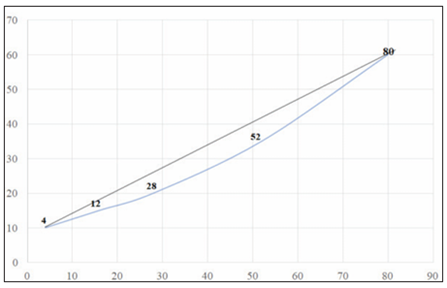
\includegraphics[width=0.7\linewidth]{imagenes/Imagen2}
		\caption{Representación del resultado de la ecuación de Regresión por Mínimos Cuadrados.}
		\label{fig:Imagen2}
	\end{figure}
	
	\section{Otras Aplicaciones del Material}
	\subsection{Regresión Lineal por Mínimos Cuadrados}
	La Regresión Lineal por Mínimos Cuadrados, debido a su simplicidad, interpretabilidad y eficacia, encuentra una amplia gama de aplicaciones en diversos campos del aprendizaje automático y el análisis de datos.\\
	\\
	Según (Wolberg, 2010), entre las aplicaciones generales de la RLMC se incluyen:\\
		
	\begin{itemize}
		\item \textbf{Análisis de Regresión Lineal:} Es la base de la regresión lineal, una herramienta fundamental en el análisis de datos para establecer relaciones lineales entre variables.
		\item \textbf{Finanzas y Economía:} Se utiliza ampliamente para predecir precios de acciones, analizar tendencias del mercado y en econometría para modelar relaciones económicas.
		\item \textbf{Procesamiento de Señales:} Se emplea para filtrar el ruido de las señales, ajustando un modelo a una señal ruidosa con el fin de minimizar el ruido y mejorar la claridad de la señal.
		\item \textbf{Procesamiento de Imágenes:} Es utilizada para mejorar o manipular imágenes, por ejemplo, eliminando ruido o afinando los bordes de los objetos para una mejor visualización o análisis.
		\item \textbf{Sistemas de Control:} Se aplica en el diseño y la optimización de sistemas de control, donde se modelan las relaciones entre entradas y salidas para predecir y ajustar el comportamiento del sistema.
		\item \textbf{Ciencias Sociales y Biología:} En un amplio rango de campos, la RLMC se emplea para modelar y predecir variables continuas, desde el crecimiento de plantas hasta el comportamiento demográfico.
	\end{itemize}
	
	Los siguientes casos de estudio específicos ilustran la aplicación de la RLMC a partir de la literatura especializada:
	\\
	\begin{itemize}
		\item \textbf{Predicción de Precios de Acciones:} Un estudio se centró en predecir el precio de cierre de acciones utilizando el método de mínimos cuadrados lineales. El documento "BBCA Stock Price Prediction Using Linear Regression Method" (Saputra \& Widiantoro, 2024), que referencia el trabajo de Emioma \& Edeki, detalla una metodología que abarca la recolección de datos históricos (precio de cierre ajustado y volumen de negociación), el preprocesamiento, la construcción del modelo de regresión lineal en la plataforma RapidMiner y la evaluación mediante métricas como el Error Cuadrático Medio (RMSE). Los hallazgos de este estudio indicaron que una división de datos del 90\% para entrenamiento y 10\% para prueba arrojó el RMSE más bajo, lo que sugiere que un tamaño de conjunto de entrenamiento suficiente es crucial para un rendimiento óptimo del modelo. Sin embargo, el RMSE resultante, aunque el más bajo entre las configuraciones probadas, aún era significativo, lo que llevó a la conclusión de que se necesitan técnicas más avanzadas para lograr una predicción fiable de los precios de las acciones en el mundo real.
		\item \textbf{Clasificación de Software:} La regresión lineal se ha utilizado para clasificar software similar, modelando la relación lineal entre datos de entrada, como vectores de diferencia de código, y una salida que indica la similitud entre programas. El modelo busca minimizar el error en los datos de entrenamiento para mejorar la precisión en la estimación de resultados para nuevos datos, lo que permite una clasificación más efectiva de software (Markovsky \& Van Huffel, 2007).
		\item \textbf{Cuantificación de la Incertidumbre en Modelos No Lineales:} La regresión por mínimos cuadrados se emplea para entrenar los parámetros de modelos de aprendizaje automático, incluyendo modelos no lineales. El método multiparamétrico delta, por ejemplo, cuantifica la incertidumbre para estos modelos, requiriendo el gradiente de la predicción del modelo y el Hessiano de la función de pérdida (la suma de errores al cuadrado) con respecto a los parámetros. Esta cuantificación es vital porque ayuda a identificar la extrapolación, es decir, las predicciones realizadas fuera del rango de los datos de entrenamiento, y a seleccionar datos de entrenamiento más adecuados o a evaluar la fiabilidad general del modelo (Miller, 2006).
	\end{itemize}
	
	La Regresión Lineal por Mínimos Cuadrados trasciende su papel como un simple modelo predictivo lineal. Su utilidad se extiende a ser un bloque constructivo fundamental para algoritmos más complejos y una herramienta diagnóstica esencial. La RLMC proporciona una base sólida para comprender las relaciones lineales, que a menudo son el punto de partida para muchas formas de modelado de datos. En el ámbito de la cuantificación de la incertidumbre, la RLMC se utiliza para entrenar los parámetros de modelos que son inherentemente no lineales. Esto significa que la minimización de los errores cuadrados sigue siendo una estrategia de optimización fundamental, incluso cuando la relación subyacente entre las variables no es una línea recta.
	\\
	Esto posiciona a la RLMC como una herramienta de diagnóstico inicial, que ayuda a identificar la complejidad del problema y la necesidad de modelos más sofisticados. Su interpretabilidad la hace particularmente valiosa para obtener una comprensión preliminar de los datos antes de recurrir a modelos de “caja negra” más complejos (Saputra \& Widiantoro, 2024).
	\\
	
\begin{thebibliography}{00}
	
	\bibitem{b1} Kaware, S. (2021). A model based linear algebraic approach for machine learning. En 2021 6th International Conference for Convergence in Technology (I2CT) (pp. 1–6). IEEE. https://doi.org/10.1109/I2CT51068.2021.9418083
	\bibitem{b2} Wolberg, J. R. (2010). Data analysis using the method of least squares: Extracting the most information from experiments. Springer.
	\bibitem{b3} Watson, G. S. (1967). Linear least squares regression. The Annals of Mathematical Statistics, 38(6), 1679–1699. https://doi.org/10.1214/aoms/1177698603
	\bibitem{b4} Menke, W. (2015). Review of the generalized least squares method. Surveys in Geophysics, 36(1), 1–25. https://doi.org/10.1007/s10712-014-9303-1
	\bibitem{b5} Andrade-Garda, J. M., \& Carlosena-Zubieta, A. (2013). Classical linear regression by the least squares method. In Basic Chemometric Techniques in Atomic Spectroscopy (pp. 29–50). Royal Society of Chemistry.
	
	\bibitem{b6} Miller, S. J. (2006). The method of least squares. Williams College.
	\bibitem{b7} Abdi, H. (2007). The method of least squares. En N. J. Salkind (Ed.), Encyclopedia of Measurement and Statistics (pp. 508–510). Sage Publications.
	\bibitem{b8} Boyko, A. A., Kukartsev, V. V., \& Tynchenko, V. S. (2020). Using linear regression with the least squares method to determine the parameters of the Solow model. IOP Conference Series: Materials Science and Engineering, 753, 032011. https://doi.org/10.1088/1757-899X/753/3/032011
	\bibitem{b9} Markovsky, I., \& Van Huffel, S. (2007). Overview of total least squares methods. Signal Processing, 87(10), 2283–2302. https://doi.org/10.1016/j.sigpro.2007.04.004
	\bibitem{b10} Saputra, S., \& Widiantoro, A. (2024). BBCA stock price prediction using linear regression method. International Journal of Artificial Intelligence and Science, 1, 25–36. https://doi.org/10.63158/IJAIS.v1.i1.7
	
\end{thebibliography}

\end{document}
